\documentclass{beamer}

\usepackage[ngerman]{babel}
\usepackage{graphicx}


% Example here:
% https://github.com/josephwright/beamer/blob/main/doc/solutions/conference-talks/conference-ornate-20min.de.tex

\mode<presentation>
{
	\usetheme{Singapore}
	%\usetheme{AnnArbor}
	%\usecolortheme{beaver}
}

\title{Kolloquium Pflichtenheft}
\subtitle{SEP WS 2021/2022}

%\titlegraphic{
\includegraphics[width=5cm]{../../docs/Pflichtenheft/graphics/LasEs-logo}}

\date{\small 2. November 2021}
\logo{
\includegraphics[width=1.5cm]{../../docs/Pflichtenheft/graphics/LasEs-logo}}

\author{\textbf{Team 2} \\ \small {Johannes Garstenauer, Stefanie Gürster, Thomas Kirz,\\ Johann Schicho, Sebastian Vogt} \normalsize}


\begin{document}

	\begin{frame}
		\titlepage
	\end{frame}

	\begin{frame}{Gliederung}
		\tableofcontents
	\end{frame}

\section{Anforderungen und Funktionalität}

\begin{frame}{Anforderungen}
	\begin{itemize}
		\item \emph{Submission und Review Management Systems}
		\pause % Durchklicken wie bei Kraftpunkt.

		\item Aufteilung in Rollen
		\begin{itemize}
			\item Nutzer
			\item Gutachter
			\item Editor
			\item Administrator
		\end{itemize}
		\pause

		\item Java mit \emph{Jakarta Server Faces}

	\end{itemize}
\end{frame}

\begin{frame}{Funktionalität}
	\begin{itemize}
		\item Verwaltung Konferenzen und Journale
		\pause
		\item Einreichungen und Gutachten
		\pause
		\item Rechte und Funktionen der Rollen
		\pause
		\item Übersicht und Verwaltung der Papers
	\end{itemize}
\end{frame}

\section{Lastenheft}
\begin{frame}{Lastenheft}
	\centering
	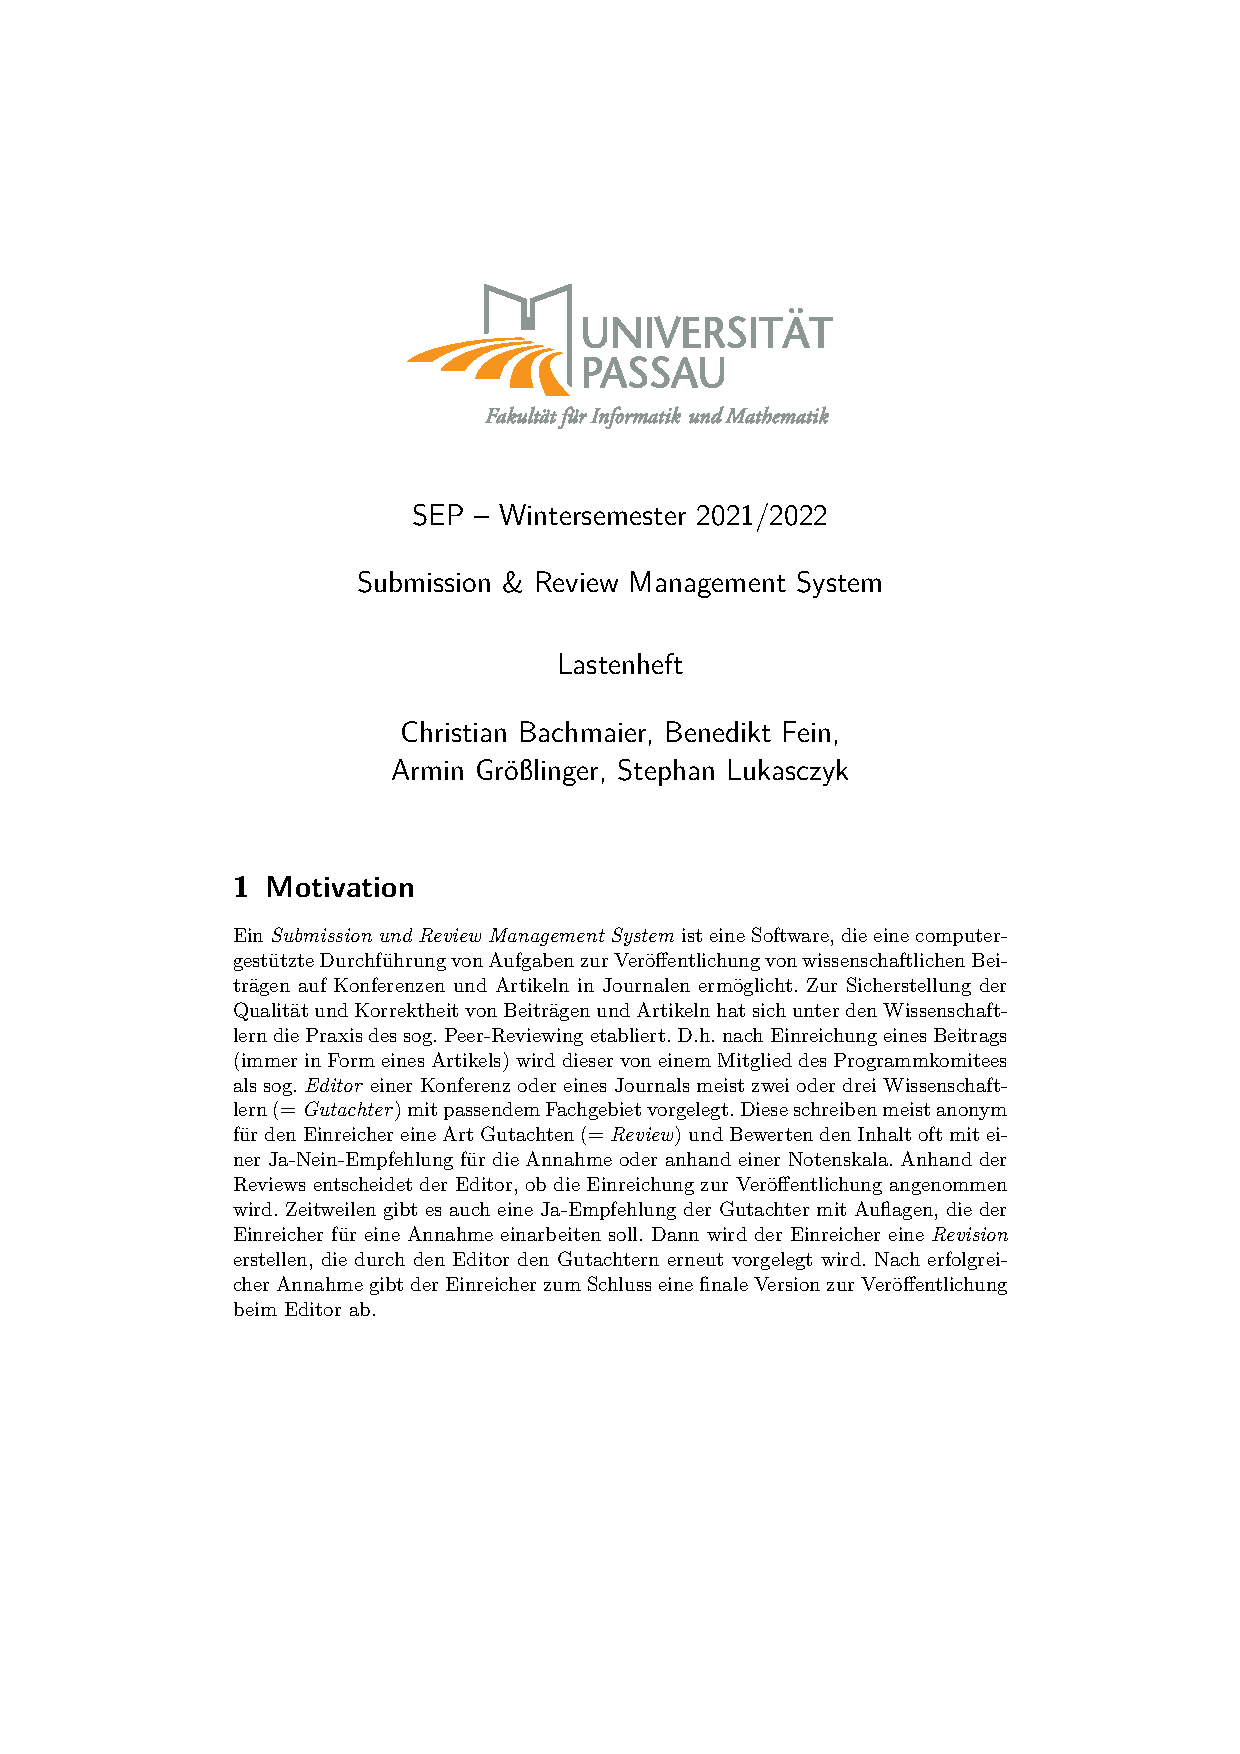
\includegraphics[height=1.1\textheight]{../../docs/Lastenheft/lastenheft}
\end{frame}


\subsection{Lücken und Unklarheiten}
\begin{frame}{Lücken und Unklarheiten}

	Fragen bei dem erste Gespräch:
	\pause

	\begin{itemize}
		\item Benachrichtigungen per E-Mail. Automatisch vs. \emph{Mailto}
		\pause
		\item Löschen eines Nutzers, kaskadierendes Löschen
		\pause
		\item Ansicht von Papers anderer Nutzer möglich?
		\pause
		\item Sind die Rollen tatsächlich hierarchisch?
	\end{itemize}

\end{frame}

\subsection{Indirekte Forderungen}
\begin{frame}{Indirekte Forderungen}
		\begin{itemize}
		\item Produktdaten
		\begin{itemize}
			\item Nutzerdaten
			\item Einreichungen
		\end{itemize}
		\pause
		\item Usability
		\begin{itemize}
			\item Gewünschte Funktionen vs. Design
			\item Suche und paginierte Listen
		\end{itemize}
		\pause
		\item Datenschutz
	\end{itemize}
\end{frame}

\section{Aussehen}
\begin{frame}{Look and Feel 1}
	\centering
	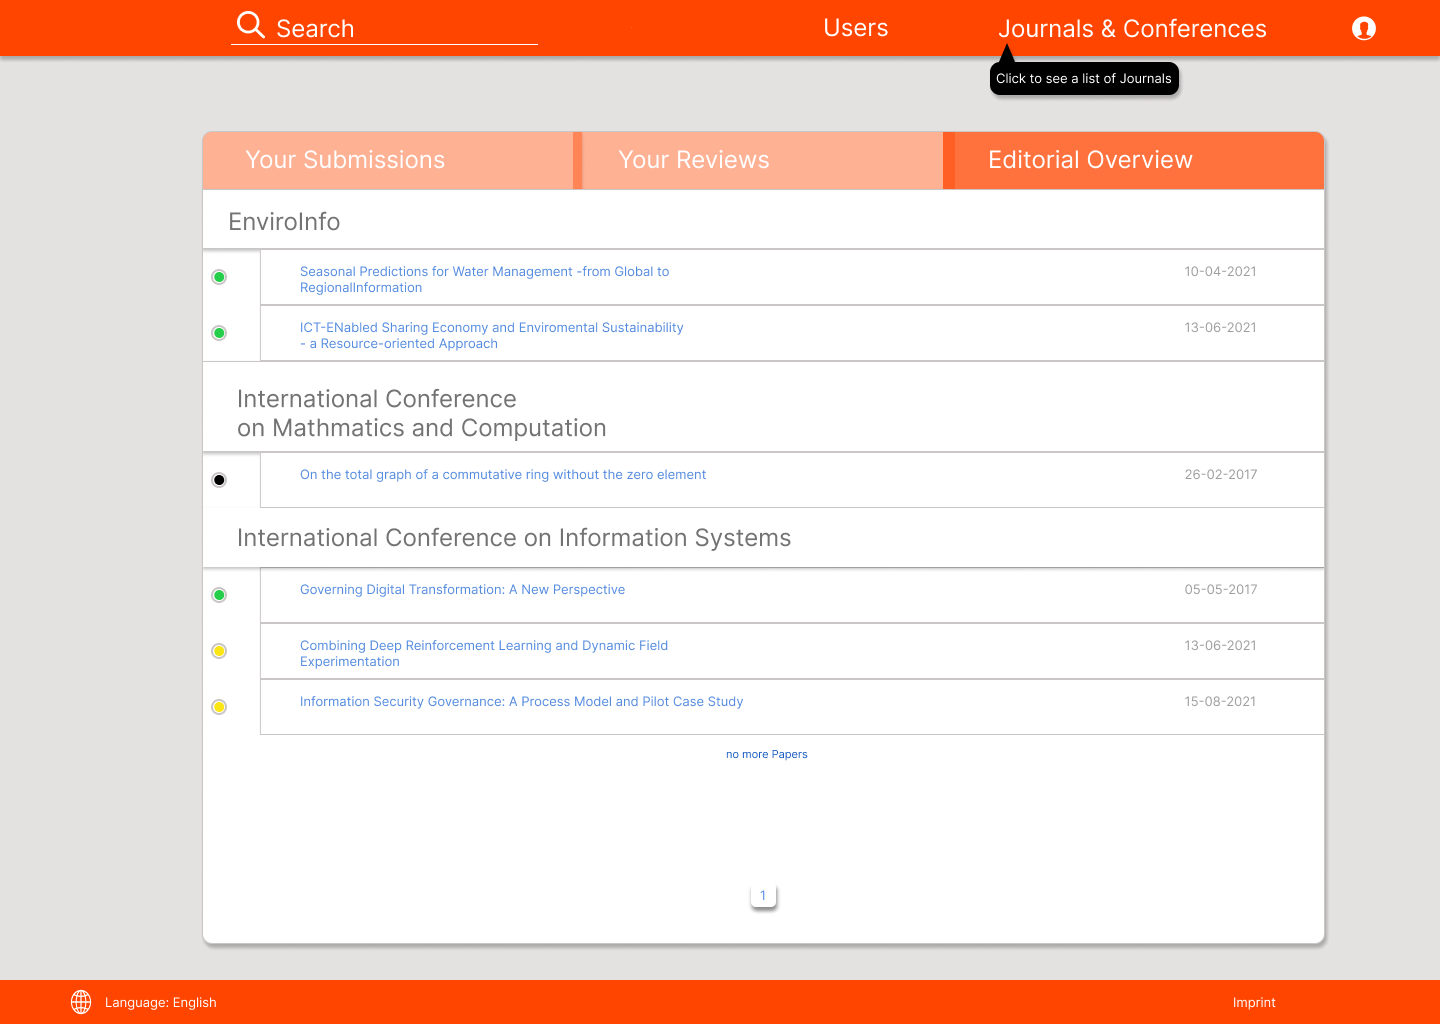
\includegraphics[height=0.9\textheight]{../../docs/Pflichtenheft/graphics/Homepage-png}
\end{frame}

\begin{frame}{Look and Feel 2}
	\centering
	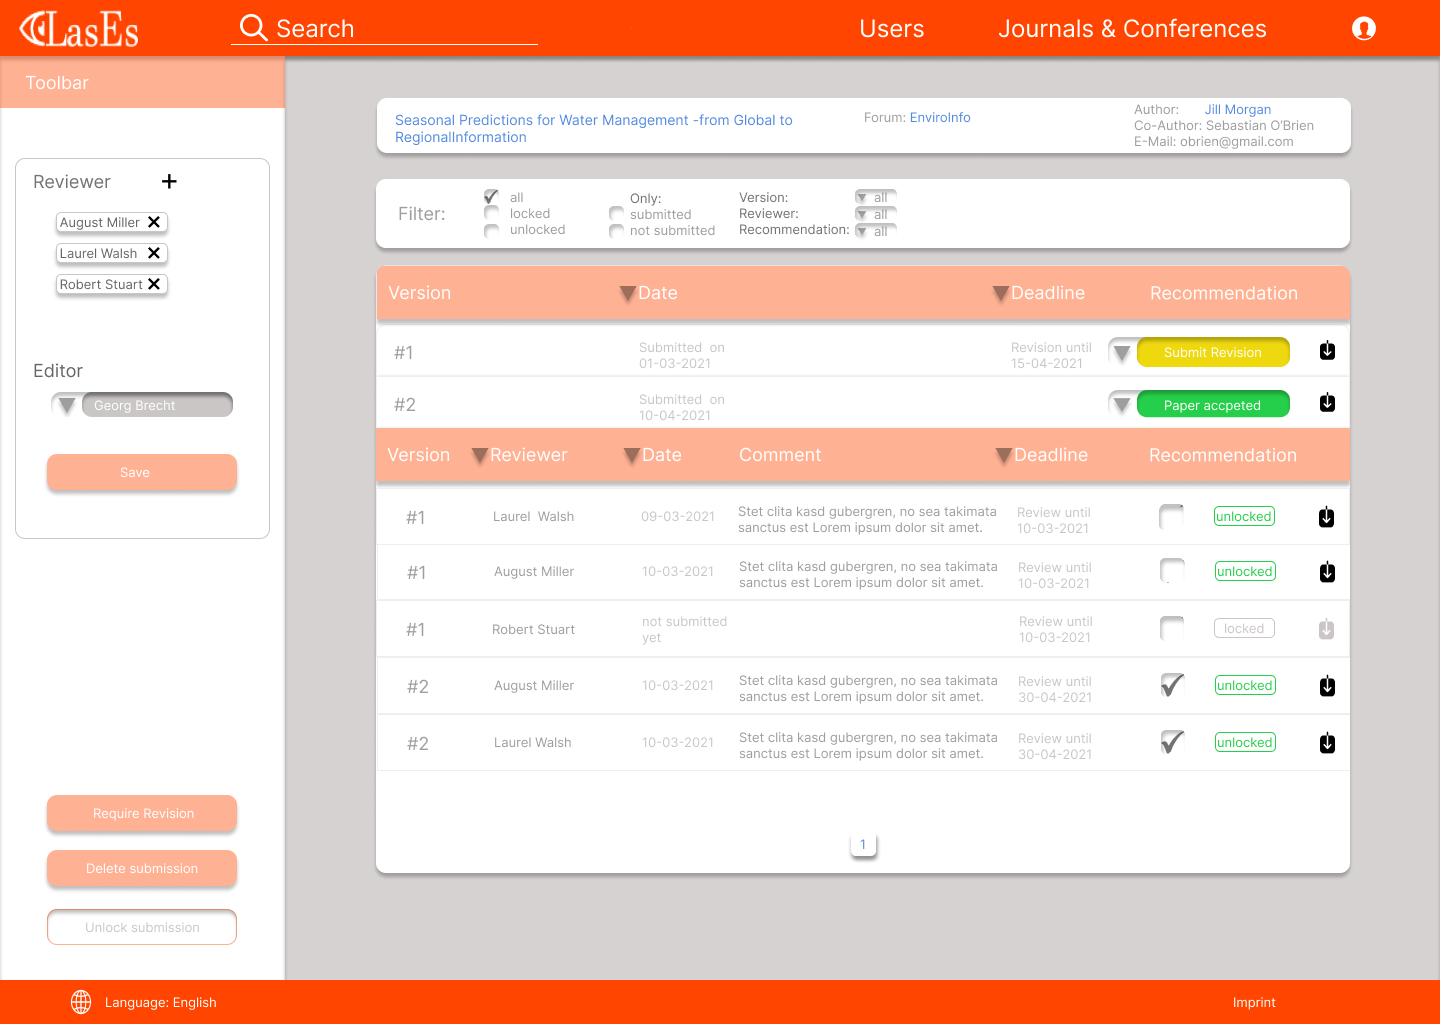
\includegraphics[height=0.9\textheight]{../../docs/Pflichtenheft/graphics/Submission-png}
\end{frame}

\section{Killer Feature}
\begin{frame}{Wieso LasEs?}
	\centering
	\pause
	\huge Benutzerfreundlichkeit
\end{frame}

\begin{frame}{Wieso LasEs?}
	\centering
	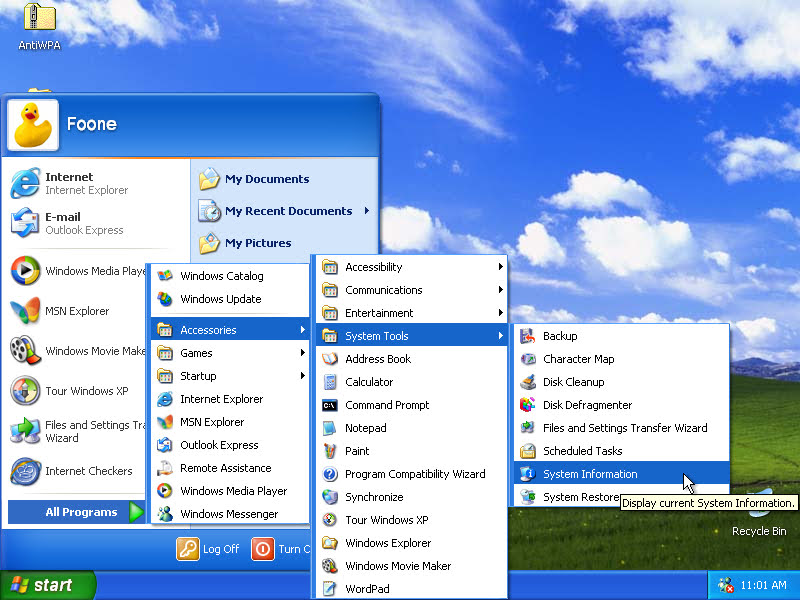
\includegraphics[height=0.8\textheight]{graphics/windowsxp}
\end{frame}

\begin{frame}{Wieso LasEs}
	\centering
	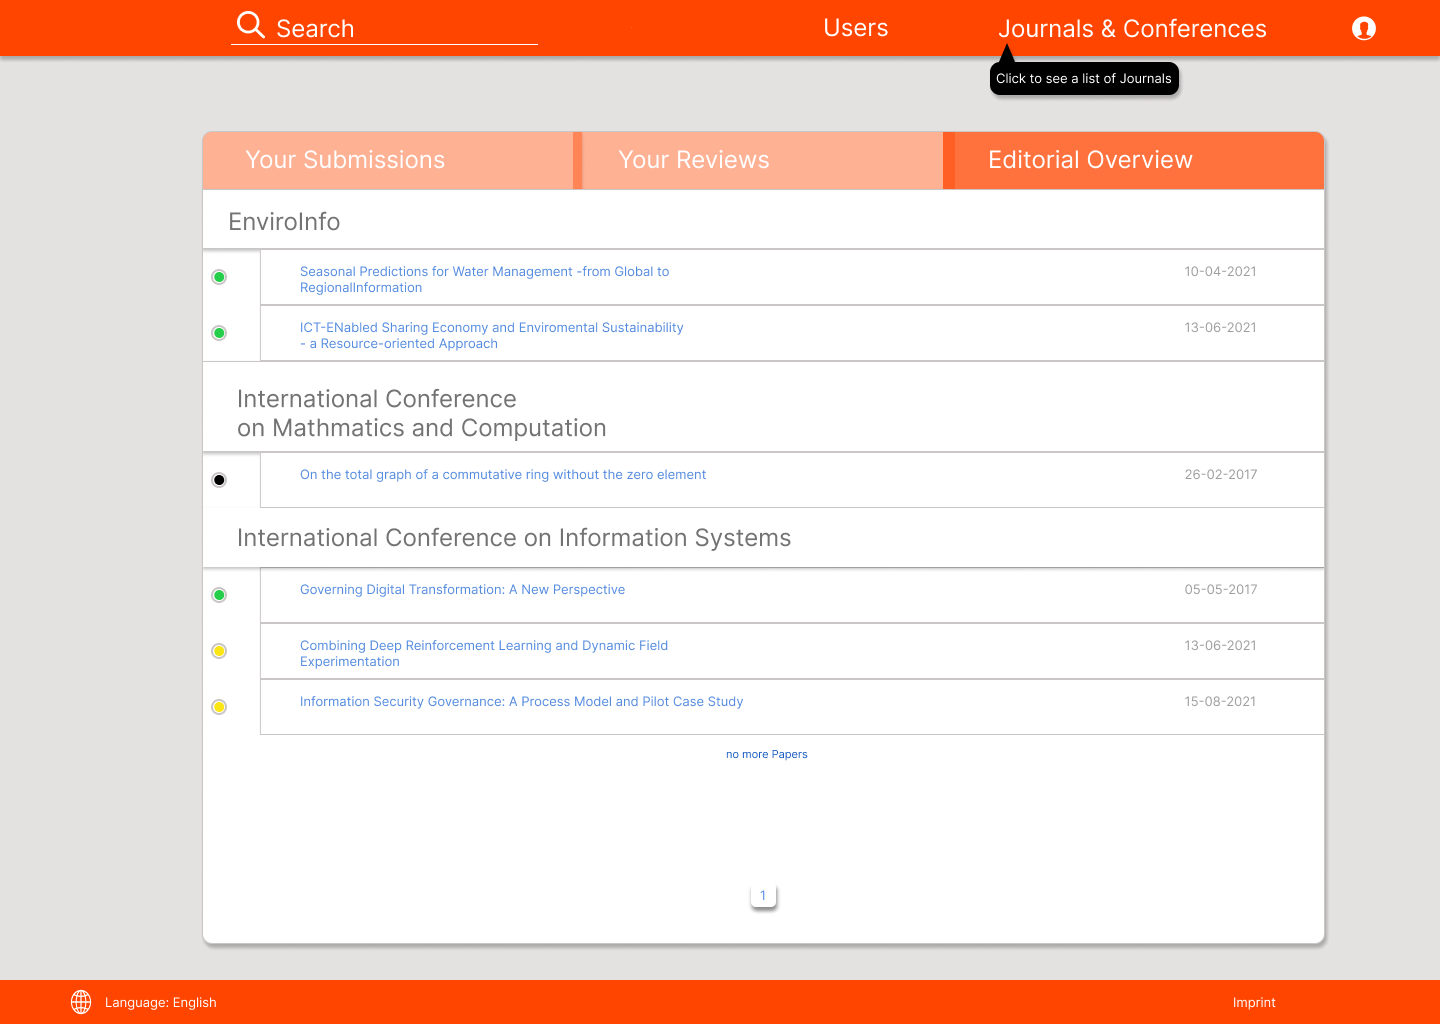
\includegraphics[height=0.75\textheight]{../../docs/Pflichtenheft/graphics/Homepage-png}
\end{frame}

\section{Navigationsstruktur}
\begin{frame}{Navigationsgraph}
	\centering
	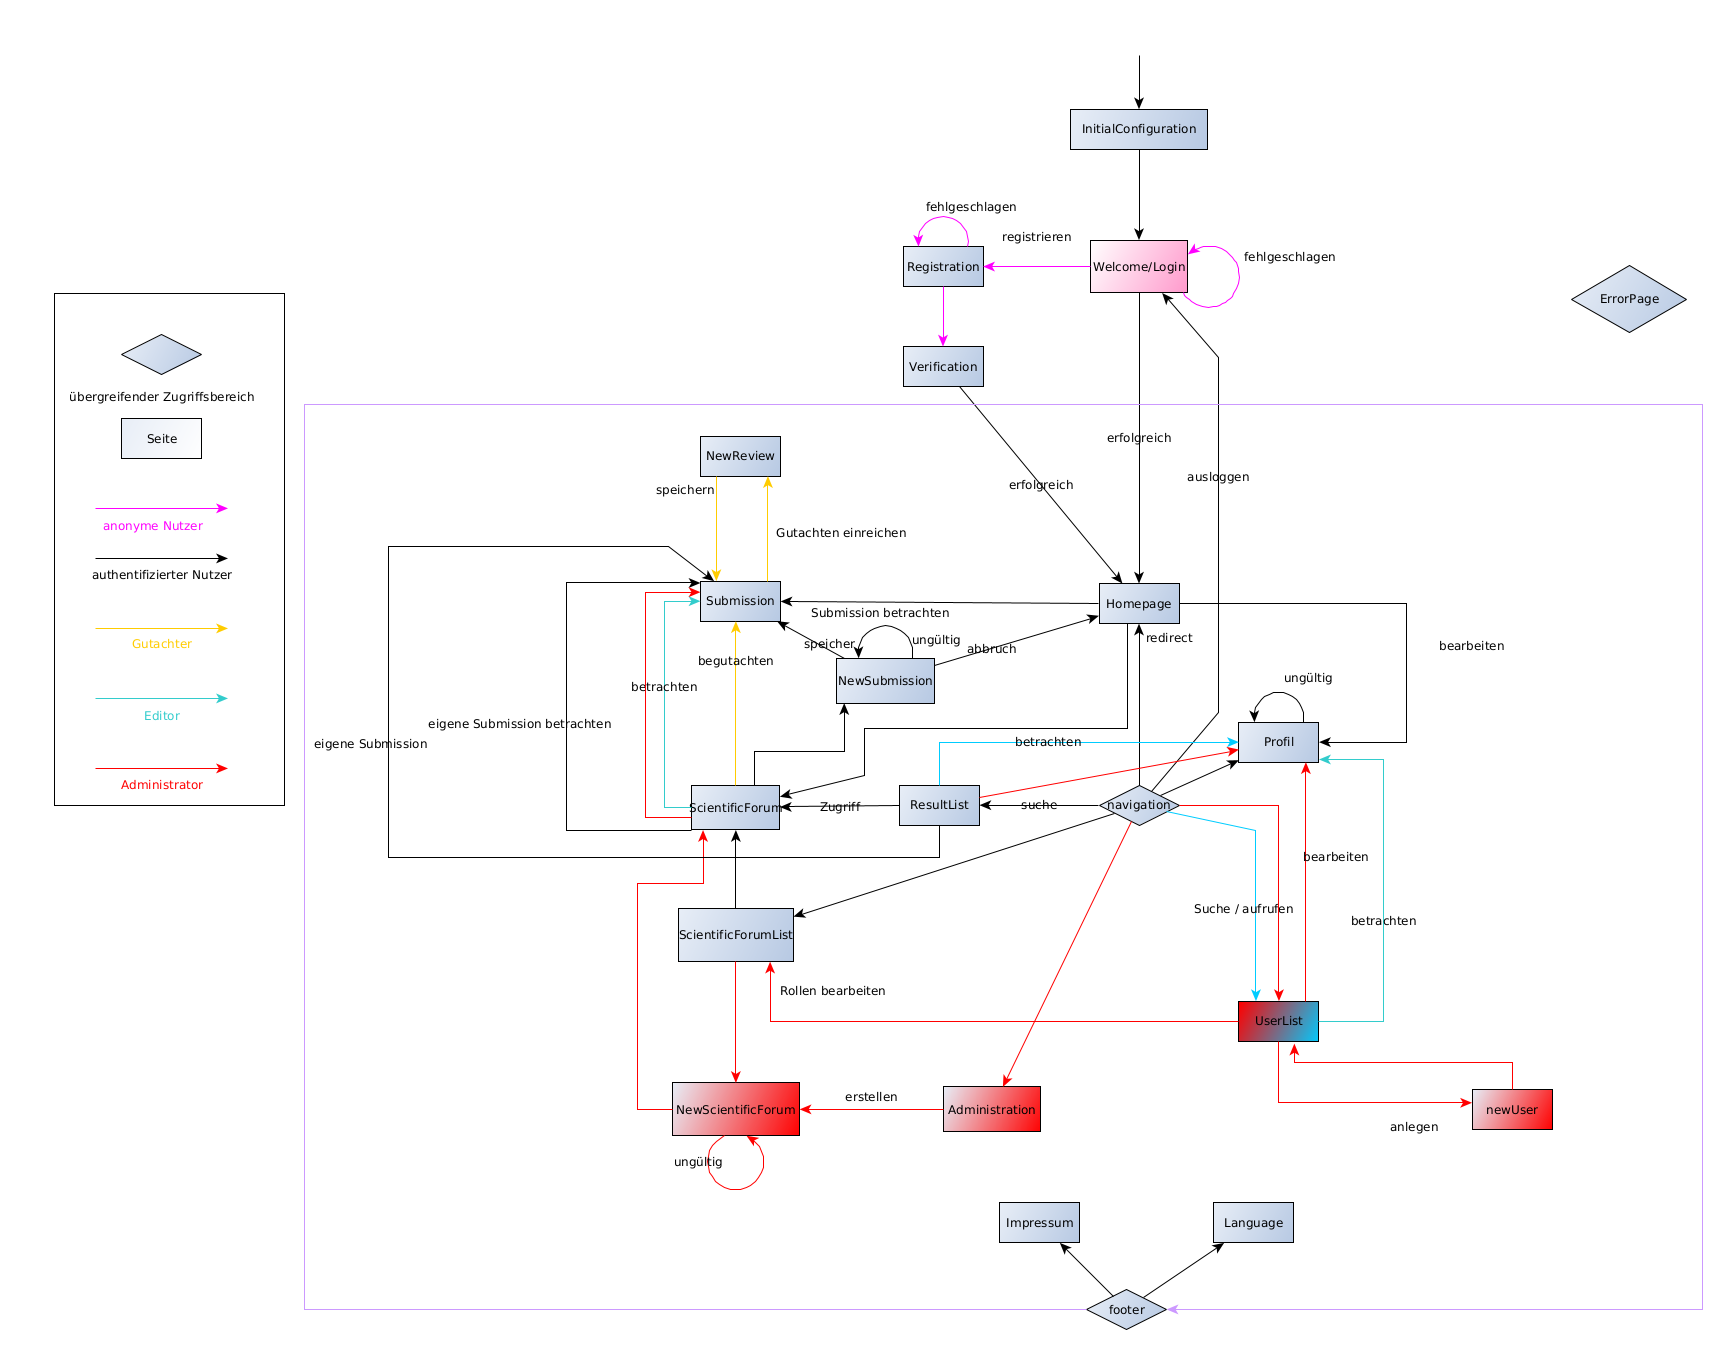
\includegraphics[height=0.8\textheight]{../../docs/Pflichtenheft/graphics/benutzerFlussyEd-png}
\end{frame}

\section{Erweiterbarkeit}

\begin{frame}{Erweiterbarkeit}
	\pause
	\begin{itemize}
		\item Gutachtervorschläge
		\pause
		\item Individuellere Personalisierung
		\pause
		\item Anforderung von Revisionen
		\pause
		\item Zurückziehen von Gutachten
		\pause
		\item Mehrsprachige Anwendung
	\end{itemize}
\end{frame}

\begin{frame}{Abgrenzungskriterien}
	\pause
	\begin{itemize}
		\item Einreichung nur in PDF
		\pause
		\item Eigene Anwendung zur Betrachtung der Paper
		\pause
		\item Keine Publikationssoftware oder Lizenzierung
		\pause
		\item Webanwendung für Desktopgeräte
	\end{itemize}
\end{frame}

\section{Testing}
\begin{frame}{Testabläufe}
	\pause
	Setup:
	\begin{itemize}
		\item mehrere Nutzer
		\item Testmodus (für E-Mailbestätigungen)
	\end{itemize}

	\pause

	Ablauf:
	\begin{itemize}
		\item Anlegen einer Konferenz
		\item Einreichung von Paper mit Koautor
		\item Koautor registriert sich später im System
		\item Editor kümmert sich um Gutachteraquirierung
		\item Abschließendes Löschen
	\end{itemize}
\end{frame}

\begin{frame}{Diskussion}
	\centering
	
\includegraphics[width=0.7\linewidth]{../../docs/Pflichtenheft/graphics/LasEs-logo}
\end{frame}

\end{document}
